\chapter{Introduction}
\section{The Standard Model}
The SM (Standard Model of particle physics) is humanity's best understanding of how the fundamental building blocks reality behave. The SM as we know it today has evolved over many years, beginning with the unification of the electromagnetic and weak forces in the late 1960's. The current evolution of the SM
includes four fundamental forces, listed in Table (TBA), and 17 fundamental particles, listed
in Table (TBA).
Calculations using the SM have been remarkably successful at making precise predictions
which have been confirmed experimentally. It is one of the most rigorously tested
theories in physics and has held up remarkably well to years of experimental testing.
\section{Quantum Chromodynamics}
In order to calculate things within the SM, we must turn to quantum field theory (QFT) to formally, mathematically describe the fundamental interactions in the SM.
In order to calculate particles interacting via the strong force, the most relevant force at the high energies provided 
by hadron-hadron collisions at RHIC, we turn to QCD. Quantum chromodynamics
introduces an additional quantum number to the SM and is governed by the SU(3) symmetry
group. This new quantum number, labeled color, can take three values referred to as
red (r), green (g), and blue (b), in an analogy to the three colors in optics. Like the electric
charge in QED, each color has an opposite, ?negative? value, carried by the antiquarks,
referred to as anti-red (�r), anti-green (�g), and anti-blue(�b).
\section{Heavy Ion Collisions}
The idea of hot hadronic matter was developed in the early 1950s by various physicists including Enrico Fermi~\cite{Fermi01071950} . 
This concept of applying statistical and hydrodynamical models to a strongly interacting particle ensemble ultimately evolved into the theory of QGP (Quark Gluon Plasma). 
Since then, systematic studies of hot hadronic matter systems have produced a greater understanding of the state of matter hypothesized to be QGP. QGP has been roughly mapped out in the hadronic phase diagram. 
The state of matter created in our laboratories is understood to be comparable to the universe about one microsecond after the big bang. And the evolution of the medium has been mapped from the initial heavy ion collision all the way to the final state particles. 

Here is the timeline overview of heavy ion collisions in general: At the moment when heavy ions collide relativistically ($\tau$=0), they are length contracted down to flat disks in the lab frame as seen in Figure .... 
Then, the initial geometry resulting from the shape of the collision overlap region and fluctuations within the nuclei is transformed into the initial energy density of the medium ($\tau$  1 fm/c). 
At that moment, the hot hadronic matter is thought to be made up of deconfined quarks and gluons in thermal equilibrium, otherwise known as QGP. 
The system then evolves hydrodynamically, expanding along the pressure gradients present in the initial energy density.
At a certain point during this expansion, the medium has cooled down enough in order to form baryons and mesons out of the quark gluon soup in a process known as hadronization. 
It is important to note that the medium is still in thermal equilibrium at this point but it is no longer known as QGP but instead as hadron gas. 
Once the medium has cooled down and expanded sufficiently, kinetic freeze-out occurs and the hadron gas becomes a group of particles which have ceased self-interaction ($\tau$  10 fm/c). 
It is this group of final state particles which can be detected much later ($\tau$  $10^{15}$ fm/c). 
Although detectable particles escape the medium at all times, the vast majority of particles we detect are produced at kinetic freeze-out. 

Although the field of high-energy nuclear physics is still evolving, several measured properties of this state of matter have come together to make QGP the prevailing explanation. Among the best observations indicating QGP are jet quenching, J/$\psi$ melting, and elliptic flow. The observation of jets measured at much lower energies than expected imply that the jets are experiencing energy loss when interacting with a strongly coupled medium. The observation of a severe reduction in the number of expected J/$\psi$ particles matches a prediction that a strongly coupled medium with a temperature above the Hagedorn temperature will melt J/$\psi$ particles. Finally, an elliptic symmetry in the angular distribution of final state particles when viewed along the beam line has been observed. The translation of initial geometry into long-range angular correlations indicates collectivity in a strongly coupled medium.
\begin{figure}
\begin{center}
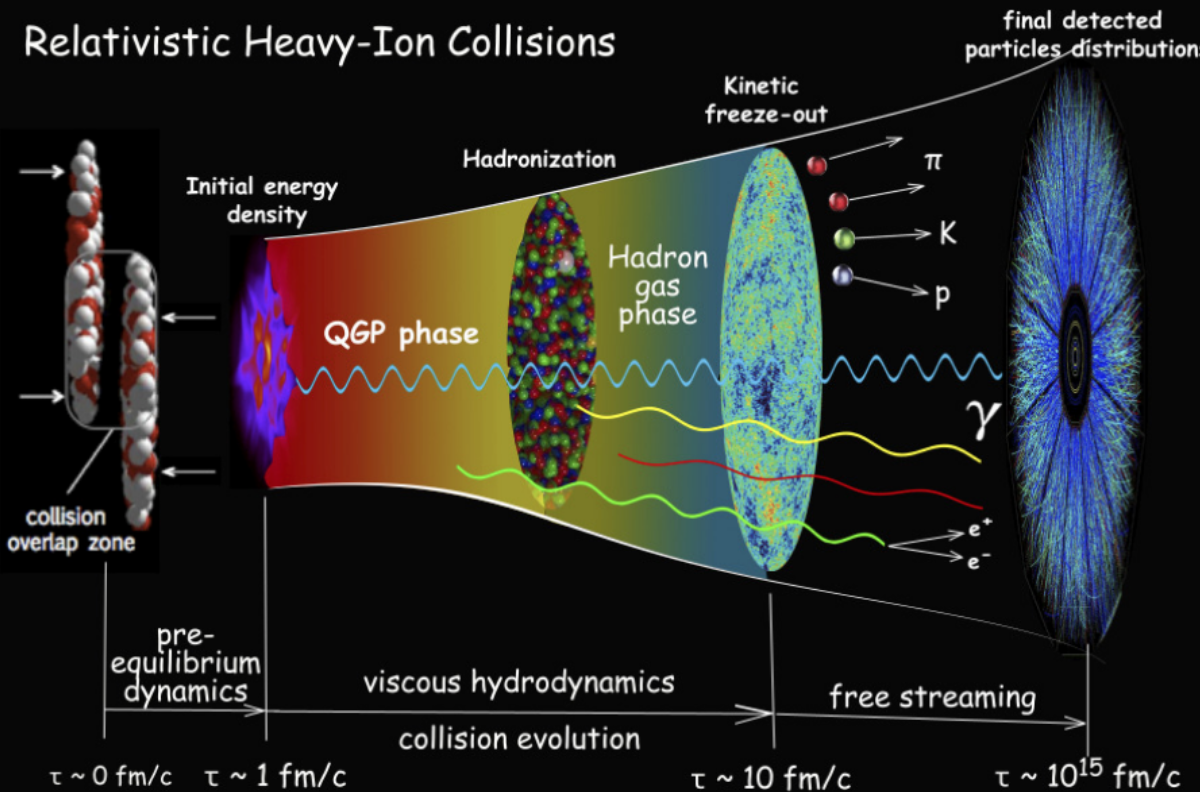
\includegraphics[width=0.55\linewidth]{figs/qgp_evolution_timeline.png}
\caption{TBA}
\end{center}
\end{figure}

